
\begin{definition}\label{def:Int_tray_vec}\textbf{Integral de trayectoria de campos vectoriales sobre trayectorias de Clase $\mathcal{C}^1$.} Sean $\boldsymbol{\sigma}:[a,b]\to A\subseteq\Rn{n}$ una trayectoria $\mathcal{C}^1$  y  $\mathbf{F}:A\subseteq\mathbb{R}^{n}\to \mathbb{R}^{n}$ un  campo vectorial continuo sobre la imagen de  $\boldsymbol{\sigma}$. Se define la \emph{integral de trayectoria del campo vectorial} $\mathbf{F}$ \emph{a lo largo de la trayectoria} $\boldsymbol{\sigma}$, y se denota por $ \int_{\boldsymbol{\sigma}} \mathbf{F}\cdot d\mathbf{s}$,  mediante
    \[
        \int_{\boldsymbol{\sigma}} \mathbf{F}\cdot d\mathbf{s}=\int_a^b     (\mathbf{F}\circ\boldsymbol{\sigma}) (t) \cdot\boldsymbol{\sigma}'(t) \, dt. 
    \]
\end{definition}

Si $\boldsymbol{\sigma}(t)$ es de clase $\mathcal{C}^1$ a trozos, se define  $\int_{\boldsymbol{\sigma}} \mathbf{F}\cdot d\mathbf{s}$ de la siguiente manera:  

\begin{definition}\label{def:Int_tray_a_trozas_vec}\textbf{Integral de trayectoria de campos vectoriales sobre trayectorias de Clase $\mathcal{C}^1$ a trozos.}    Sean $\boldsymbol{\sigma}:[a,b]\to A\subseteq\Rn{n}$ una trayectoria $\mathcal{C}^1$  a trozos y  $\mathbf{F}:A\subseteq\mathbb{R}^{n}\to \mathbb{R}^{n}$ un  campo vectorial continuo sobre la imagen de  $\boldsymbol{\sigma}$.   Se define la \emph{integral de trayectoria del campo vecorial} $\mathbf{F}$ \emph{a lo largo de la trayectoria} $\boldsymbol{\sigma}$,  y se  denota por $\int_{\boldsymbol{\sigma}} \mathbf{F}\cdot d\mathbf{s}$, mediante
  
    \[
       \int_{\boldsymbol{\sigma}} \mathbf{F}\cdot d\mathbf{s}  =\sum_{i=0}^{m-1}\int_{I_i}  (\mathbf{F} \circ\boldsymbol{\sigma})(t) \cdot \boldsymbol{\sigma}'(t) \:dt,  
    \]
    donde $ I_i= (t_i, t_{i+1})$,  $\boldsymbol{\sigma}\lvert_{I_i}$ es de clase $\mathcal{C}^1$  y  $\{t_i\}_{i=0}^{m}$  es una partici\'on de $I$.
\end{definition}


 \begin{tarea}Sean $\mathbf{F}(x,y) =  (y, 2xy +1) $  y  $\boldsymbol{\sigma}: [-1,1]\to\Rn{2}\;  : \sigma(t) = ( t^{2}, t^{2})$,  calcular,   $$\int_{\sigma}\mathbf{F}\cdot d\mathbf{s}$$
\end{tarea}


\begin{definition}\label{def:trabajo_fuer_constante}\textbf{Trabajo realizado por una fuerza constante sobre un objeto que se mueve en l\'inea recta.}  
Sea un objeto que se desplaza desde un punto $A$ hasta un punto $B$ por el segmento que los une y  bajo la acci\'on de una fuerza \(\mathbf{F}\) constante. 
Se define el     \emph{trabajo realizado por la fuerza sobre el objeto} como:
\[
W = \mathbf{F} \cdot \mathbf{d} = \|\mathbf{F}\| \, \|\mathbf{d}\| \, \cos\theta,
\]
donde
\begin{itemize} 
\item $\mathbf{d} = B - A$ es el vector de desplazamiento del objeto. 
\item $\|\mathbf{F}\|$ es la magnitud (o norma) de la fuerza.
\item $\|\mathbf{d}\|$ es la magnitud (o norma) del desplazamiento.
\item $\theta$ es el ángulo comprendido entre el vector fuerza y el vector desplazamiento. 
\end{itemize} 
\end{definition}



\textbf{Interpretaci\'on física:} El trabajo representa la cantidad de energ\'ia transferida al objeto por la fuerza en la direcci\'on del desplazamiento. Dependiendo del ángulo $\theta$, se presentan tres casos fundamentales:
\begin{itemize}
    \item Si \(0 \leq \theta < 90^\circ\), el trabajo es positivo: la fuerza ayuda al movimiento.
    \item Si \(90^\circ < \theta \leq 180^\circ\), el trabajo es negativo: la fuerza se opone al movimiento.
    \item Si \(\theta = 90^\circ\), el trabajo es cero: la fuerza no realiza trabajo sobre el objeto.
\end{itemize}

% ==========================================
% DIAGRAMA FÍSICO DEL TRABAJO MECÁNICO
% ==========================================

\begin{figure}[htbp]
    \centering
    % Llamamos al archivo con el código TikZ extraído
    \begin{center} 
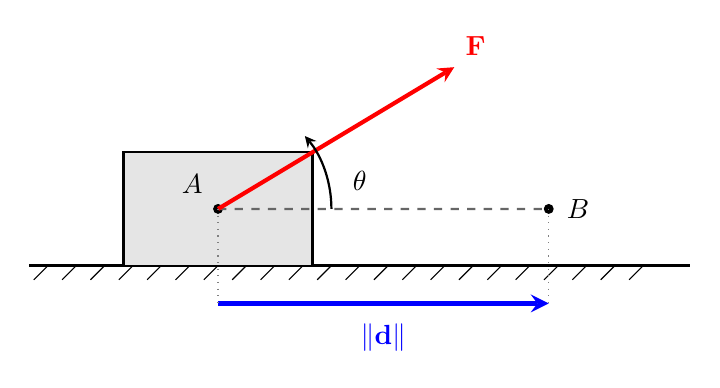
\begin{tikzpicture}[scale=1.2, >=stealth] 

    % 1. Piso / Superficie de apoyo con textura
    \draw[line width=1pt] (-1,0) -- (6,0); 
    \foreach \x in {-0.8,-0.5,...,5.8} {
        \draw (\x,0) -- (\x-0.15,-0.15); 
    }

    % 2. Bloque / Objeto en gris
    \draw[thick, fill=gray!20] (0,0) rectangle (2,1.2); 
    
    % Centro de masa (Punto A: Posición inicial del objeto)
    \coordinate (CM) at (1,0.6); 
    \fill[black] (CM) circle (1.5pt) node[above left=2pt] {$A$}; 

    % 3. Línea auxiliar horizontal (Dirección del movimiento)
    \draw[dashed, black!60, thick] (CM) -- (4.5,0.6); 
    
    % Punto B: Posición final del centro de masa del objeto tras el desplazamiento
    \fill[black] (4.5,0.6) circle (1.5pt) node[right=3pt] {$B$};

    % 4. Vector Fuerza F saliendo de A
    \draw[->, line width=1.5pt, red] (CM) -- (3.5,2.1) node[above right] {$\mathbf{F}$}; 

    % 5. Ángulo theta entre la fuerza y la dirección del movimiento
    \draw[thick, black, ->] (2.2,0.6) arc (0:40:1.2); 
    \node at (2.5,0.9) {$\theta$}; 

    % 6. Vector Desplazamiento posicionado en el suelo (Une las proyecciones de A y B)
    \draw[->, line width=1.8pt, blue] (1, -0.4) -- (4.5, -0.4) node[midway, below=3pt] {$\|\mathbf{d}\|$}; 
    
    % Líneas de proyección tenues que nacen en los puntos A y B hacia el suelo
    \draw[dotted, black!50] (1,0.6) -- (1,-0.4);
    \draw[dotted, black!50] (4.5,0.6) -- (4.5,-0.4);

\end{tikzpicture} 
\end{center} 
    \label{fig:interpretacion fisica}
\end{figure}


\begin{obs}
\textbf{Dependencia del sentido del movimiento.}
Es importante notar que el trabajo es una magnitud que depende intrínsecamente del sentido en el que se recorre el segmento. Si un objeto se desplaza en sentido inverso (desde $B$ hacia $A$), el nuevo vector de desplazamiento es $\mathbf{d}' = A - B = -\mathbf{d}$.  Al calcular el trabajo $W'$ en este recorrido inverso bajo la misma fuerza constante $\mathbf{F}$, obtenemos:
\[ W' = \mathbf{F} \cdot \mathbf{d}' = \mathbf{F} \cdot (-\mathbf{d}) = -(\mathbf{F} \cdot \mathbf{d}) = -W \]
Físicamente, esto significa que si una fuerza realiza un trabajo positivo al acompañar el movimiento en un sentido, realizará exactamente el mismo trabajo pero con signo negativo (se opondrá) si el objeto realiza el camino de regreso. Esta propiedad fundamental se preservará luego al generalizar el concepto mediante la integral de línea.
\end{obs}





\begin{example} 
Un objeto se desplaza desde el punto $A = (0, 0)$ hasta el punto $B = (3, 0)$ a lo largo del segmento que los une, bajo la acción de la fuerza constante $\mathbf{F} = (2, 1)$. Calcular el trabajo realizado por $\mathbf{F}$ sobre el objeto. 

\noindent\textbf{Solución:} Para calcular el trabajo realizado bajo una fuerza constante a lo largo de un segmento rectilíneo, aplicamos la Definición \ref{def:trabajo_fuer_constante}. 
Para ello, en primer lugar, hallamos el vector de desplazamiento $\mathbf{d}$ restando las coordenadas del punto final y el punto inicial:
\[ 
\mathbf{d} = B - A = (3, 0) - (0, 0) = (3, 0). 
\] 
A continuación, siguiendo,  planteamos el producto escalar entre el vector fuerza $\mathbf{F}$ y el vector desplazamiento $\mathbf{d}$:
$$
W = \mathbf{F} \cdot \mathbf{d} = (2, 1) \cdot (3, 0) = 6.
$$
Por lo tanto, el trabajo realizado por la fuerza sobre el objeto es igual a $6$. Como $W > 0$, la fuerza favorece el movimiento; esto concuerda físicamente con el hecho de que el ángulo ($\theta$ entre $\mathbf{F}$ y $\mathbf{d}$ es agudo ($\theta < 90^\circ$). \hfill $\blacksquare$
\end{example}







% =========================================================================
% CONSTRUCCIÓN ANALÍTICA DE LA INTEGRAL DE LÍNEA (TRABAJO MECÁNICO)
% =========================================================================

\subsection*{Construcción Geométrica y Analítica de la Integral de Línea}

Para la siguiente deducci\'on se tendrá en cuenta el caso en el cual $\boldsymbol{\sigma} : [a, b] \to A \subseteq \mathbb{R}^n$ es una trayectoria de clase $\mathcal{C}^1$ y  $\mathbf{F} : A \subseteq \mathbb{R}^n \to \mathbb{R}^n$  es un campo vectorial continuo. Se deja al lector escribir el caso en el cual $\boldsymbol{\sigma}$ es una trayectoria de clase $\mathcal{C}^1$ a trozos. 

\subsubsection*{1. Partición del intervalo paramétrico y discretización}
Sea  $P$   una partición regular del intervalo cerrado $[a, b]$ definida por el conjunto ordenado de puntos $\{t_0, t_1, \dots, t_m\}$ de modo que:
\[
a = t_0 < t_1 < t_2 < \dots < t_i < t_{i+1} < \dots < t_m = b
\]
Esta partición divide al intervalo $ [a, b]$ en $m$ subintervalos de la forma $[t_i, t_{i+1}]$, cada uno con una longitud constante dada por \[\Delta t = t_{i+1} - t_i=\dfrac{b-a}{m} \quad \forall \:  0 \leq  t \leq m.\] Geométricamente, esta partición en  $[a, b]$  induce una subdivisión sobre la trayectoria curva $C =\boldsymbol{\sigma}([a,b])$ en el espacio $\mathbb{R}^n$, delimitada por los puntos de posición discretos $\boldsymbol{\sigma}(t_0), \boldsymbol{\sigma}(t_1), \dots, \boldsymbol{\sigma}(t_m)$.


\subsubsection*{2. Aproximación del desplazamiento y de la fuerza en un subintervalo}
Analicemos el trabajo elemental realizado por el campo sobre el objeto al desplazarse a lo largo del arco de curva que conecta $\boldsymbol{\sigma}(t_i)$ con $\boldsymbol{\sigma}(t_{i+1})$. Si la amplitud del subintervalo $\Delta t_i$ es suficientemente pequeña, dicho arco puede aproximarse mediante el segmento rectilíneo lineal $\mathbf{d}$  que define el desplazamiento neto del tramo, 
\[
\mathbf{d}_i  = \boldsymbol{\sigma}(t_{i+1}) - \boldsymbol{\sigma}(t_i)
\]
Por otra parte, debido a la continuidad asumida para el campo vectorial $\mathbf{F}$, la fuerza que actúa sobre el cuerpo a lo largo de este intervalo local permanece aproximadamente invariable. En consecuencia, es lícito aproximar su valor mediante el campo evaluado en el extremo inferior del subintervalo, esto es, $\mathbf{F}(\boldsymbol{\sigma}(t_i))$. Así, el trabajo elemental $W_i$ efectuado en este tramo se modela a través del producto escalar:
\[
W_i \approx \mathbf{F}(\boldsymbol{\sigma}(t_i)) \cdot \big(  \boldsymbol{\sigma}(t_{i+1}) -  \boldsymbol{\sigma}(t_i) \big)
\]


\subsubsection*{3. Linealización mediante el Teorema del Valor Medio por componentes} 
Dado que la trayectoria $\boldsymbol{\sigma}(t) = \big(\sigma_1(t), \sigma_2(t), \dots, \sigma_n(t)\big)$ es una función vectorial de clase  $\mathcal{C}^1$ , podemos aplicar el Teorema del Valor Medio clásico de una variable a cada una de sus funciones componentes escalares de forma independiente en el subintervalo $[t_i, t_{i+1}]$. Este Teorema garantiza la existencia de puntos intermedios $t^k_i \in (t_i, t_{i+1})$ tales que:
\[
\sigma_k(t_{i+1}) - \sigma_k(t_i) = \sigma_k'(t^k_i)(t_{i+1} - t_i) = \sigma_k'(t^k_i) \Delta t, \quad \text{para cada } k = 1, 2, \dots, n.
\]
Al considerar una partición infinitamente fina, los puntos intermedios convergen al extremo local ($t^k_i \to t_i$). Así, al agrupar nuevamente las componentes en forma de vector, la diferencia de posición se aproxima en términos del vector velocidad $\boldsymbol{\sigma}'(t_i)$ y del paso del parámetro:
\[ 
\boldsymbol{\sigma}(t_{i+1}) - \boldsymbol{\sigma}(t_i) \approx \boldsymbol{\sigma}'(t_i) \Delta t. 
\] 
Al sustituir esta aproximación lineal en la ecuación del trabajo elemental, se obtiene una formulación analítica que depende de manera directa del incremento del parámetro: 
\[ 
W_i \approx \mathbf{F}(\boldsymbol{\sigma}(t_i)) \cdot \boldsymbol{\sigma}'(t_i) \Delta t. 
\] 


\subsubsection*{4. Suma de Riemann y convergencia al límite integral} 
De este modo, obtenemos una primera aproximación al trabajo total $W$ realizado por el campo de fuerzas a lo largo de toda la trayectoria mediante la acumulación de las contribuciones elementales de cada subintervalo, lo cual da lugar a una estructura formal de suma de Riemann: 
\[ 
W \approx \sum_{i=0}^{m-1} W_i = \sum_{i=0}^{m-1} \mathbf{F}(\boldsymbol{\sigma}(t_i)) \cdot \boldsymbol{\sigma}'(t_i) \Delta t. 
\] 

Con base en el análisis anterior, \textbf{definimos formalmente el trabajo realizado por la fuerza variable} como el paso al límite de la suma de Riemann cuando el número de subdivisiones de la partición regular tiende a infinito ($m \to +\infty$): 
\[ 
W = \lim_{m \to +\infty} \sum_{i=0}^{m-1} \mathbf{F}(\boldsymbol{\sigma}(t_i)) \cdot \boldsymbol{\sigma}'(t_i) \Delta t. 
\] 
Dado que el campo vectorial $\mathbf{F}$ es continuo y la trayectoria $\boldsymbol{\sigma}$ es de clase $\mathcal{C}^1$, la función resultante del producto escalar $\mathbf{F}(\boldsymbol{\sigma}(t)) \cdot \boldsymbol{\sigma}'(t)$ es una función escalar continua en el intervalo cerrado $[a,b]$ y, por ende, integrable en el sentido de Riemann. Así, el límite de la suma converge formalmente hacia la integral definida sobre el intervalo paramétrico: 
\[ 
W = \int_a^b \mathbf{F}(\boldsymbol{\sigma}(t)) \cdot \boldsymbol{\sigma}'(t) \, dt. \tag*{$\blacksquare$}
\]
Teniendo en cuenta la Definición \ref{def:Int_tray_a_trozas_vec}  llegamos a la siguiente definic\'on formal

\begin{definition}\label{def:trabajo_trayectoria}\textbf{Trabajo de un campo de fuerzas sobre una trayectoria.} 
Sea $\boldsymbol{\sigma} : [a, b] \to A \subseteq \mathbb{R}^n$ una trayectoria de clase $\mathcal{C}^1$ a trozos y sea $\mathbf{F} : A \subseteq \mathbb{R}^n \to \mathbb{R}^n$ un campo vectorial continuo. Se define el \emph{trabajo realizado por el campo $\mathbf{F}$ sobre la trayectoria $\boldsymbol{\sigma}$}, y se denota por $W$, mediante:
\[ 
W = \int_{\boldsymbol{\sigma}} \mathbf{F} \cdot d\mathbf{s}  
\] 
\end{definition}


\begin{example} \textbf{Dependencia de la orientación.}
 Calcular  el trabajo realizado por el campo \( \mathbf{F}(x, y) = (x, 0) \)  sobre el segmento geométrico del eje $x$  que une los puntos $(0,0)$ y $(1,0)$,   analizando el comportamiento de la integral al recorrerlo en sentidos opuestos.
\end{example}

\noindent\textbf{Solución:} Por un lado, llamemos $W_1$ al trabajo realizado por el campo  $\mathbf{F}$  sobre el segmento si lo recorremos con orientación desde $(0,0)$ hacia $(1,0)$.  Para ello consideremos
\[ \boldsymbol{\sigma}_1(t) = (t, 0), \quad t \in [0, 1] \]

Calculamos su vector derivada:
\[ \boldsymbol{\sigma}_1'(t) = (1, 0) \]

Evaluamos el campo $\mathbf{F}$ sobre la trayectoria sustituyendo $x = t$ e $y = 0$:
\[ \mathbf{F}(\boldsymbol{\sigma}_1(t)) = (t, 0) \]

Calculamos el trabajo $W_1$:
\[ W_1 = \int_{\boldsymbol{\sigma}_1} \mathbf{F} \cdot d\mathbf{s} = \int_{0}^{1} (t, 0) \cdot (1, 0) \, dt = \int_{0}^{1} t \, dt = \left[ \frac{t^2}{2} \right]_{0}^{1} = \frac{1}{2} \]

Por otro lado, llamemos $W_2$ al trabajo realizado por el campo  $\mathbf{F}$  sobre el segmento recorrido de manera inversa, es decir,  con orientación desde $(1,0)$ hacia $(0,0)$.  Para ello consideremos
\[ \boldsymbol{\sigma}_2(t) = (1-t, 0), \quad t \in [0, 1] \]

Calculamos su vector derivada:
\[ \boldsymbol{\sigma}_2'(t) = (-1, 0) \]

Evaluamos el campo $\mathbf{F}$ sobre esta trayectoria sustituyendo $x = 1-t$ e $y = 0$:
\[ \mathbf{F}(\boldsymbol{\sigma}_2(t)) = (1-t, 0) \]

Calculamos el trabajo $W_2$:
\[ W_2 = \int_{\boldsymbol{\sigma}_2} \mathbf{F} \cdot d\mathbf{s} = \int_{0}^{1} (1-t, 0) \cdot (-1, 0) \, dt = \int_{0}^{1} (t-1) \, dt = \left[ \frac{t^2}{2} - t \right]_{0}^{1} = -\frac{1}{2} \]

Como podemos observar, $W_1 = -W_2$.  Esto ilustra de manera explícita que:
\[ \int_{\boldsymbol{\sigma}_1} \mathbf{F} \cdot d\mathbf{s} = -\int_{\boldsymbol{\sigma}_2} \mathbf{F} \cdot d\mathbf{s} \]

Por lo tanto, al invertir el sentido en el que se recorre la trayectoria, el valor absoluto de la integral de línea se mantiene constante, pero \emph{su signo cambia}.







\begin{obs}\label{obs:orientacion_vectorial}
El Ejemplo anterior introduce una de las propiedades más importantes de las integrales de línea de campos vectoriales: \textbf{la dependencia de la orientación}.  A diferencia de los campos escalares, donde el sentido del recorrido no altera el valor de la integral (ver Observación~\ref{obs:param}), en campos vectoriales el signo del trabajo cambia por completo si invertimos el sentido del movimiento. 
\end{obs}


